\documentclass[12pt]{article}
\usepackage{float}
\usepackage{graphicx}
\usepackage[font=small,labelfont=bf]{caption}

\pagestyle{empty}
\setcounter{tocdepth}{4}
\setcounter{secnumdepth}{4}

\topmargin=0cm
\oddsidemargin=0cm
\textheight=22.0cm
\textwidth=16cm
\parindent=0cm
\parskip=0.15cm
\topskip=0truecm
\raggedbottom
\abovedisplayskip=3mm
\belowdisplayskip=3mm
\abovedisplayshortskip=0mm
\belowdisplayshortskip=2mm
\normalbaselineskip=12pt
\normalbaselines

\begin{document}

\vspace*{0.5in}
\centerline{\bf\Large Design Document - Iteration 2}

\vspace*{0.5in}
\centerline{\bf\Large Team PA-PI-a}

\vspace*{0.5in}
\centerline{\bf\Large 18 March 2018}

\vspace*{1.5in}
\begin{table}[htbp]
\caption{Team}
\begin{center}
\begin{tabular}{|r | c|}
\hline
Name & ID Number \\
\hline\hline
Melanie Taing & 40009850 \\
Laurie Gagnon & 22943433 \\
Wayne Yiel Leung & 26586988 \\
Jordan Rutty & 27300107 \\
Alice Barkhouse & 27486782 \\
Michael Foo & 40000225 \\
Pierre-Andre Leger & 40004010 \\
Colin Greczkowski & 40001600 \\
\hline
\end{tabular}
\end{center}
\end{table}

\clearpage

\tableofcontents

\clearpage

\section{Introduction}
\textit {From the template (delete me) --- The introduction of the document provides an overview of the entire document, briefly introducing what are its goals, and what information is to be found in it.}

\section{Architectural Design} \label{sec:arch}

\textit {From the template (delete me) --- This section must give a high-level description of the system in terms of its modules and their respective purpose and exact interfaces.}

\subsection{Architectural Diagram}

\textit {From the template (delete me) --- A UML class diagram or package diagram depicting the high-level structure of the system, accompanied by a one-paragraph text describing the rationale of this design. It is mandatory that the system be divided into at least two subsystems, and that the purpose of each of these subsystems be exposed here.}

\subsection{Subsystem Interface Specifications}

\textit {From the template (delete me) --- Specification of the software interfaces between the subsystems, i.e. specific messages (or function calls) that are exchanged by the subsystems. These are also often called ``Module Interface Specifications''.
Description of the parameters to be passed into these function calls in order to have a service fulfilled, including valid and invalid ranges of values. Each subsystem interface must be presented in a separate subsection.}

\section{Detailed Design} \label{sec:detail}

\textit {From the template (delete me) --- Complete description of the system design, describing one subsystem separately in respective subsection. UML class diagrams are to be used, as well as a short textual description describing the purpose of each class.}

\subsection{Subsystem X}

\subsubsection{Detailed Design Diagram}

\textit {From the template (delete me) --- UML class diagram depicting the internal structure of the subsystem, accompanied by a paragraph of text describing the rationale of this design.}

\subsubsection{Units Description}


\paragraph {AbstractAppController.java}
\begin{center}
\footnotesize
\begin{tabular}{|l|l|}
\hline
\textbf{Class Name }   & {AbstractAppController.java} \\ \hline
\textbf {Inherits from} & {~} \\ \hline
\textbf {Description}   & {Abstract App Controller} \\ \hline
\textbf {Attributes} & ~ \\ \hline
\textbf {Methods} & 

\footnotesize
\begin{tabular}{l|l|l|l}
\textbf{Visibility} & \textbf{Method Name} & \textbf{Return type} &\textbf{Description} \\ \hline
public &AbstractAppController &~&Constructor\\ \hline
public &start &void &Abstract start class\\ \hline
public &shutdown&void &Abstract shutdown class\\ \hline
public &run &void &Abstract run class\\
\end{tabular} \\ \hline

\end{tabular}
\end{center}

\paragraph {AbstractEventListener.java}
\begin{center}
\footnotesize
\begin{tabular}{|l|l|}
\hline
\textbf {Class Name} & {AbstractEventListener.java} \\ \hline 
\textbf {Inherits from} & { java.awt.event.ActionListener} \\ \hline 
\textbf {Description} & { Abstract Event Listener} \\ \hline 
\textbf {Attributes} &

\footnotesize
\begin{tabular}{l|l|l|l}
\textbf{Visibility} & \textbf{Data type} & \textbf{Name} & \textbf{Description} \\ \hline
package& AbstractView & view & ~  \\ \hline
package & AbstractViewController & controller & ~
\end{tabular} \\ \hline
\textbf {Methods} &

\footnotesize
\begin{tabular}{l|l|l|p{3.0cm}}
\vspace*{0.1cm}
\textbf{Visibility} & \textbf{Method Name} & \textbf{Return type} &\textbf{Description} \\ \hline
public &AbstractEventListener&~ &Constructor \\ \hline 
public &setView &void&Setter for view \\ \hline 
public &getView &AbstractView &Getter for view \\ \hline 
public&setController &void&Setter for controller \\ \hline 
public &getController&AbstractViewController&Getter for controller \\ \hline 
public &actionPerformed&void&Default message to implement this method in the view controller

\end{tabular} \\ \hline

\end{tabular}
\end{center}

\paragraph {AbstractModel.java}
\begin{center}
\footnotesize
\begin{tabular}{|l|l|}
\hline
\textbf {Class Name} & {AbstractModel.java} \\ \hline 
\textbf {Inherits From} & {} \\ \hline 
\textbf {Description} & { Abstract class for models} \\ \hline 
\textbf {Attributes} &

\footnotesize
\begin{tabular}{l|l|l|l}
\textbf{Visibility} & \textbf{Data type} & \textbf{Name} & \textbf{Description} \\ \hline
package&boolean &boolNew&used to determine if id has been set \\ \hline
private & HashSet\textless AbstractView\textgreater & m\textunderscore views & stores the views \\
\end{tabular} \\ \hline
\textbf {Methods} &

\footnotesize
\begin{tabular}{l|l|l|l}
\textbf{Visibility} & \textbf{Method Name} & \textbf{Return type} &\textbf{Description} \\ \hline
public &isNew&boolean &getter for boolNew \\ \hline 
public &setIsNewModel&void&setter for boolNew \\ \hline 
public &setView &void &setter for views \\ \hline 
public &removeView &void &deletes views \\ \hline 
public &notifyViews&void &calls for update on all views
\end{tabular} \\ \hline

\end{tabular}
\end{center}

\paragraph {AbstractView.java}
\begin{center}
\footnotesize
\begin{tabular}{|l|l|}
\hline
\textbf {Class Name} & {AbstractView.java} \\ \hline 
\textbf {Inherits From} & {} \\ \hline 
\textbf {Description} & { Abstract view class} \\ \hline 
\textbf {Attributes} & ~ \\ \hline
\textbf {Methods} &

\footnotesize
\begin{tabular}{l|l|l|l}
\textbf{Visibility} & \textbf{Method Name} & \textbf{Return type} &\textbf{Description} \\ \hline
package&AbstractView &Constructor \\ \hline 
public&update &void&abstract update class
\end{tabular} \\ \hline

\end{tabular}
\end{center}
\paragraph {AbstractViewController.java}
\begin{center}
\footnotesize
\begin{tabular}{|l|l|}
\hline
\textbf {Class Name} & {AbstractViewController.java} \\ \hline 
\textbf {Inherits From} & {} \\ \hline 
\textbf {Description} & { Abstract class for view controller} \\ \hline 
\textbf {Attributes} &

\footnotesize
\begin{tabular}{l|l|l|p{5.8cm}}
\textbf{Visibility} & \textbf{Data type} & \textbf{Name} & \textbf{Description} \\ \hline
package &AbstractView &view &primary view \\ \hline 
package &AbstractView &secondaryView&secondary view \\ \hline 
private &boolean &controllerInitialized&determines if the controller has been initialized
\end{tabular} \\ \hline
\textbf {Methods} &

\footnotesize
\begin{tabular}{l|l|l|l}
\textbf{Visibility} & \textbf{Method Name} & \textbf{Return type} &\textbf{Description} \\ \hline
public&AbstractViewController&~&constructor \\ \hline 
public&setView&void&Setter for view \\ \hline 
public&getView&AbstractView &Getter for view \\ \hline 
public&setSecondaryView&void&Setter for secondary view \\ \hline 
public&getSecondaryView&AbstractView &Getter for secondary view \\ \hline 
public&setIsInitialized&void&Setter for controllerInitialized \\ \hline 
public&getIsInitialized&boolean&getter for controllerInitialized
\end{tabular} \\ \hline

\end{tabular}
\end{center}
\paragraph {AccountController.java}
\paragraph {AccountList.java}
\paragraph {AccountMap.java}
\paragraph {AccountModel.java}
\paragraph {AccountRepository.java}
\paragraph {AccountTransactionRepository.java}
\paragraph {AccountView.java}
\paragraph {Database.java}
\paragraph {DummyAppController.java}
\paragraph {ImportTransaction.java}
\paragraph {Iteration2AppController.java}
\paragraph {Main.java}
\paragraph {MainController.java}
\paragraph {MainView.java}
\paragraph {SQLStringFactory.java}
\paragraph {SQLValueMap.java}
\paragraph {TransactionController.java}
\paragraph {TransactionList.java}
\paragraph {TransactionMap.java}
\paragraph {TransactionModel.java}
\paragraph {TransactionRepository.java}
\paragraph {TransactionView.java}
\paragraph {UserModel.java}
\paragraph {Util.java}

\section{Dynamic Design Scenarios}

\subsubsection{Adding an account}

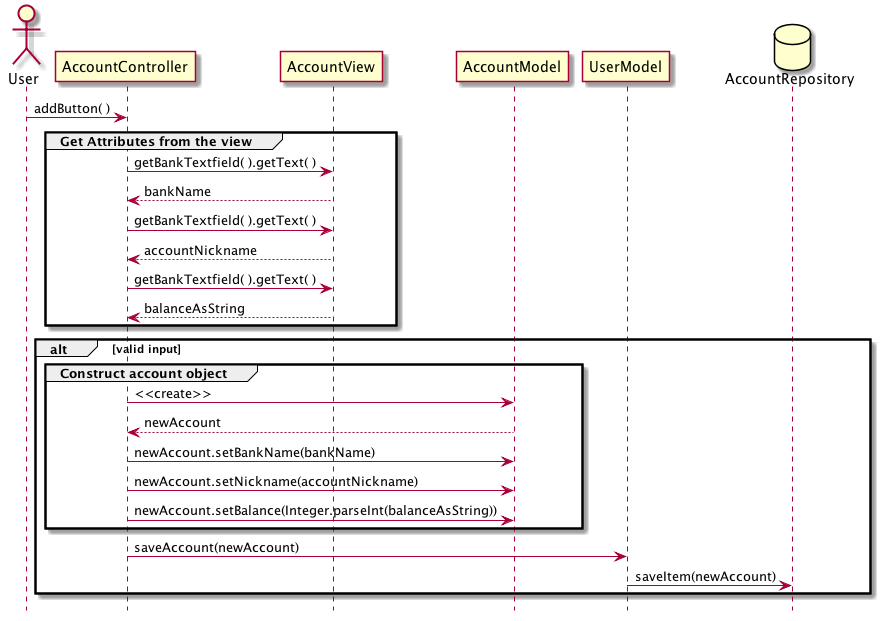
\includegraphics[width=\textwidth,height=\textheight,keepaspectratio]{diagrams/sequence/addAccount.png}
\captionof{figure}{Adding an account}

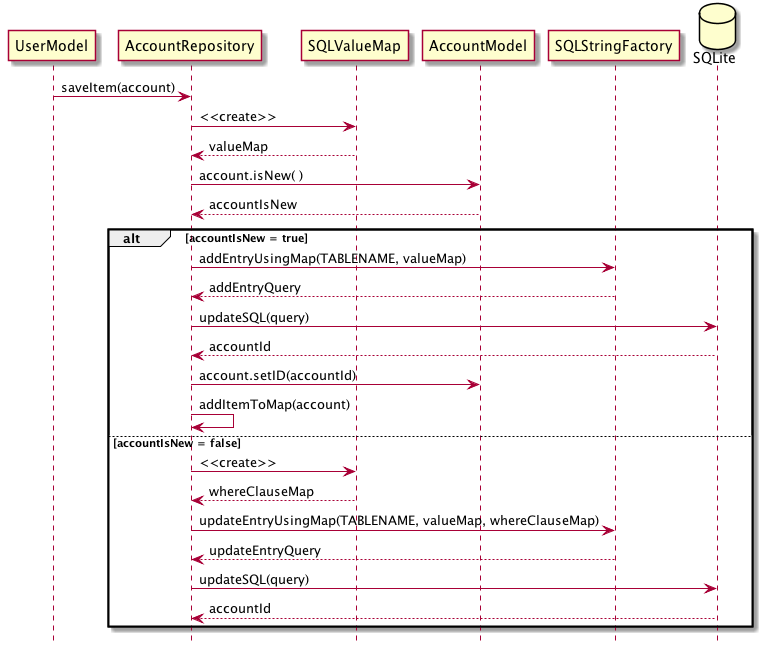
\includegraphics[width=\textwidth,height=\textheight,keepaspectratio]{diagrams/sequence/accRepoSaveItem.png}
\captionof{figure}{AccountRepository saving an account}

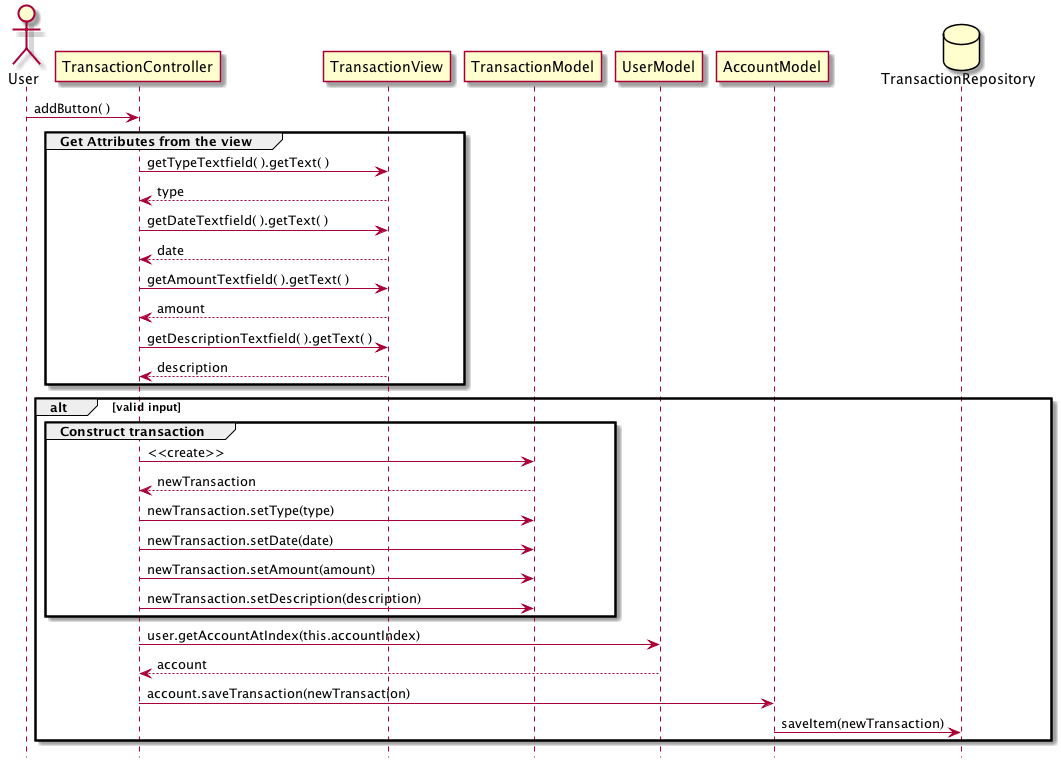
\includegraphics[width=\textwidth,height=\textheight,keepaspectratio]{diagrams/sequence/addTransaction.png}
\captionof{figure}{Adding a transaction}

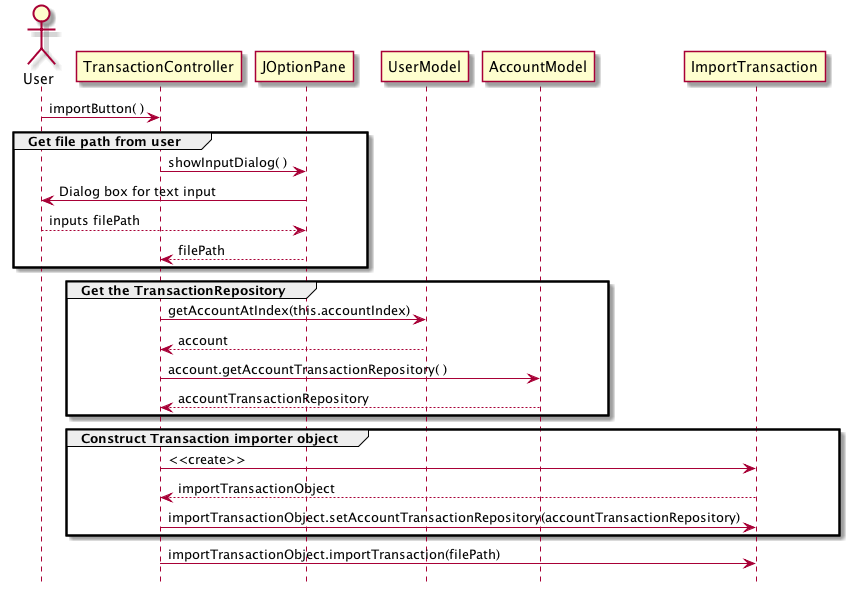
\includegraphics[width=\textwidth,height=\textheight,keepaspectratio]{diagrams/sequence/importTransaction.png}
\captionof{figure}{Importing a transaction}

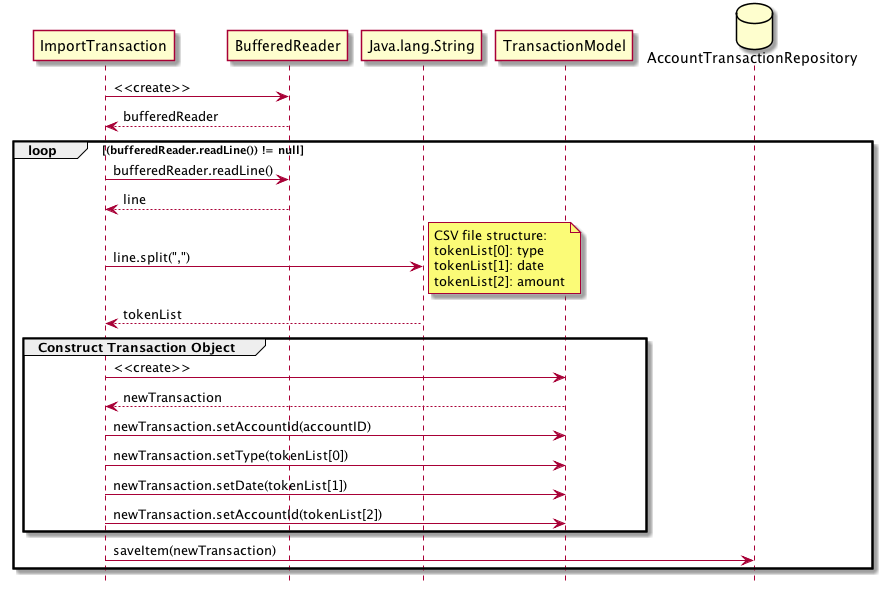
\includegraphics[width=\textwidth,height=\textheight,keepaspectratio]{diagrams/sequence/importTransaction2.png}
\captionof{figure}{Importing a transaction (cont.)}



\end{document}
